
\documentclass{article} % For LaTeX2e
\usepackage{iclr2021_conference,times}

% Optional math commands from https://github.com/goodfeli/dlbook_notation.
%%%%% NEW MATH DEFINITIONS %%%%%

\usepackage{amsmath,amsfonts,bm}

% Mark sections of captions for referring to divisions of figures
\newcommand{\figleft}{{\em (Left)}}
\newcommand{\figcenter}{{\em (Center)}}
\newcommand{\figright}{{\em (Right)}}
\newcommand{\figtop}{{\em (Top)}}
\newcommand{\figbottom}{{\em (Bottom)}}
\newcommand{\captiona}{{\em (a)}}
\newcommand{\captionb}{{\em (b)}}
\newcommand{\captionc}{{\em (c)}}
\newcommand{\captiond}{{\em (d)}}

% Highlight a newly defined term
\newcommand{\newterm}[1]{{\bf #1}}


% Figure reference, lower-case.
\def\figref#1{figure~\ref{#1}}
% Figure reference, capital. For start of sentence
\def\Figref#1{Figure~\ref{#1}}
\def\twofigref#1#2{figures \ref{#1} and \ref{#2}}
\def\quadfigref#1#2#3#4{figures \ref{#1}, \ref{#2}, \ref{#3} and \ref{#4}}
% Section reference, lower-case.
\def\secref#1{section~\ref{#1}}
% Section reference, capital.
\def\Secref#1{Section~\ref{#1}}
% Reference to two sections.
\def\twosecrefs#1#2{sections \ref{#1} and \ref{#2}}
% Reference to three sections.
\def\secrefs#1#2#3{sections \ref{#1}, \ref{#2} and \ref{#3}}
% Reference to an equation, lower-case.
\def\eqref#1{equation~\ref{#1}}
% Reference to an equation, upper case
\def\Eqref#1{Equation~\ref{#1}}
% A raw reference to an equation---avoid using if possible
\def\plaineqref#1{\ref{#1}}
% Reference to a chapter, lower-case.
\def\chapref#1{chapter~\ref{#1}}
% Reference to an equation, upper case.
\def\Chapref#1{Chapter~\ref{#1}}
% Reference to a range of chapters
\def\rangechapref#1#2{chapters\ref{#1}--\ref{#2}}
% Reference to an algorithm, lower-case.
\def\algref#1{algorithm~\ref{#1}}
% Reference to an algorithm, upper case.
\def\Algref#1{Algorithm~\ref{#1}}
\def\twoalgref#1#2{algorithms \ref{#1} and \ref{#2}}
\def\Twoalgref#1#2{Algorithms \ref{#1} and \ref{#2}}
% Reference to a part, lower case
\def\partref#1{part~\ref{#1}}
% Reference to a part, upper case
\def\Partref#1{Part~\ref{#1}}
\def\twopartref#1#2{parts \ref{#1} and \ref{#2}}

\def\ceil#1{\lceil #1 \rceil}
\def\floor#1{\lfloor #1 \rfloor}
\def\1{\bm{1}}
\newcommand{\train}{\mathcal{D}}
\newcommand{\valid}{\mathcal{D_{\mathrm{valid}}}}
\newcommand{\test}{\mathcal{D_{\mathrm{test}}}}

\def\eps{{\epsilon}}


% Random variables
\def\reta{{\textnormal{$\eta$}}}
\def\ra{{\textnormal{a}}}
\def\rb{{\textnormal{b}}}
\def\rc{{\textnormal{c}}}
\def\rd{{\textnormal{d}}}
\def\re{{\textnormal{e}}}
\def\rf{{\textnormal{f}}}
\def\rg{{\textnormal{g}}}
\def\rh{{\textnormal{h}}}
\def\ri{{\textnormal{i}}}
\def\rj{{\textnormal{j}}}
\def\rk{{\textnormal{k}}}
\def\rl{{\textnormal{l}}}
% rm is already a command, just don't name any random variables m
\def\rn{{\textnormal{n}}}
\def\ro{{\textnormal{o}}}
\def\rp{{\textnormal{p}}}
\def\rq{{\textnormal{q}}}
\def\rr{{\textnormal{r}}}
\def\rs{{\textnormal{s}}}
\def\rt{{\textnormal{t}}}
\def\ru{{\textnormal{u}}}
\def\rv{{\textnormal{v}}}
\def\rw{{\textnormal{w}}}
\def\rx{{\textnormal{x}}}
\def\ry{{\textnormal{y}}}
\def\rz{{\textnormal{z}}}

% Random vectors
\def\rvepsilon{{\mathbf{\epsilon}}}
\def\rvtheta{{\mathbf{\theta}}}
\def\rva{{\mathbf{a}}}
\def\rvb{{\mathbf{b}}}
\def\rvc{{\mathbf{c}}}
\def\rvd{{\mathbf{d}}}
\def\rve{{\mathbf{e}}}
\def\rvf{{\mathbf{f}}}
\def\rvg{{\mathbf{g}}}
\def\rvh{{\mathbf{h}}}
\def\rvu{{\mathbf{i}}}
\def\rvj{{\mathbf{j}}}
\def\rvk{{\mathbf{k}}}
\def\rvl{{\mathbf{l}}}
\def\rvm{{\mathbf{m}}}
\def\rvn{{\mathbf{n}}}
\def\rvo{{\mathbf{o}}}
\def\rvp{{\mathbf{p}}}
\def\rvq{{\mathbf{q}}}
\def\rvr{{\mathbf{r}}}
\def\rvs{{\mathbf{s}}}
\def\rvt{{\mathbf{t}}}
\def\rvu{{\mathbf{u}}}
\def\rvv{{\mathbf{v}}}
\def\rvw{{\mathbf{w}}}
\def\rvx{{\mathbf{x}}}
\def\rvy{{\mathbf{y}}}
\def\rvz{{\mathbf{z}}}

% Elements of random vectors
\def\erva{{\textnormal{a}}}
\def\ervb{{\textnormal{b}}}
\def\ervc{{\textnormal{c}}}
\def\ervd{{\textnormal{d}}}
\def\erve{{\textnormal{e}}}
\def\ervf{{\textnormal{f}}}
\def\ervg{{\textnormal{g}}}
\def\ervh{{\textnormal{h}}}
\def\ervi{{\textnormal{i}}}
\def\ervj{{\textnormal{j}}}
\def\ervk{{\textnormal{k}}}
\def\ervl{{\textnormal{l}}}
\def\ervm{{\textnormal{m}}}
\def\ervn{{\textnormal{n}}}
\def\ervo{{\textnormal{o}}}
\def\ervp{{\textnormal{p}}}
\def\ervq{{\textnormal{q}}}
\def\ervr{{\textnormal{r}}}
\def\ervs{{\textnormal{s}}}
\def\ervt{{\textnormal{t}}}
\def\ervu{{\textnormal{u}}}
\def\ervv{{\textnormal{v}}}
\def\ervw{{\textnormal{w}}}
\def\ervx{{\textnormal{x}}}
\def\ervy{{\textnormal{y}}}
\def\ervz{{\textnormal{z}}}

% Random matrices
\def\rmA{{\mathbf{A}}}
\def\rmB{{\mathbf{B}}}
\def\rmC{{\mathbf{C}}}
\def\rmD{{\mathbf{D}}}
\def\rmE{{\mathbf{E}}}
\def\rmF{{\mathbf{F}}}
\def\rmG{{\mathbf{G}}}
\def\rmH{{\mathbf{H}}}
\def\rmI{{\mathbf{I}}}
\def\rmJ{{\mathbf{J}}}
\def\rmK{{\mathbf{K}}}
\def\rmL{{\mathbf{L}}}
\def\rmM{{\mathbf{M}}}
\def\rmN{{\mathbf{N}}}
\def\rmO{{\mathbf{O}}}
\def\rmP{{\mathbf{P}}}
\def\rmQ{{\mathbf{Q}}}
\def\rmR{{\mathbf{R}}}
\def\rmS{{\mathbf{S}}}
\def\rmT{{\mathbf{T}}}
\def\rmU{{\mathbf{U}}}
\def\rmV{{\mathbf{V}}}
\def\rmW{{\mathbf{W}}}
\def\rmX{{\mathbf{X}}}
\def\rmY{{\mathbf{Y}}}
\def\rmZ{{\mathbf{Z}}}

% Elements of random matrices
\def\ermA{{\textnormal{A}}}
\def\ermB{{\textnormal{B}}}
\def\ermC{{\textnormal{C}}}
\def\ermD{{\textnormal{D}}}
\def\ermE{{\textnormal{E}}}
\def\ermF{{\textnormal{F}}}
\def\ermG{{\textnormal{G}}}
\def\ermH{{\textnormal{H}}}
\def\ermI{{\textnormal{I}}}
\def\ermJ{{\textnormal{J}}}
\def\ermK{{\textnormal{K}}}
\def\ermL{{\textnormal{L}}}
\def\ermM{{\textnormal{M}}}
\def\ermN{{\textnormal{N}}}
\def\ermO{{\textnormal{O}}}
\def\ermP{{\textnormal{P}}}
\def\ermQ{{\textnormal{Q}}}
\def\ermR{{\textnormal{R}}}
\def\ermS{{\textnormal{S}}}
\def\ermT{{\textnormal{T}}}
\def\ermU{{\textnormal{U}}}
\def\ermV{{\textnormal{V}}}
\def\ermW{{\textnormal{W}}}
\def\ermX{{\textnormal{X}}}
\def\ermY{{\textnormal{Y}}}
\def\ermZ{{\textnormal{Z}}}

% Vectors
\def\vzero{{\bm{0}}}
\def\vone{{\bm{1}}}
\def\vmu{{\bm{\mu}}}
\def\vtheta{{\bm{\theta}}}
\def\va{{\bm{a}}}
\def\vb{{\bm{b}}}
\def\vc{{\bm{c}}}
\def\vd{{\bm{d}}}
\def\ve{{\bm{e}}}
\def\vf{{\bm{f}}}
\def\vg{{\bm{g}}}
\def\vh{{\bm{h}}}
\def\vi{{\bm{i}}}
\def\vj{{\bm{j}}}
\def\vk{{\bm{k}}}
\def\vl{{\bm{l}}}
\def\vm{{\bm{m}}}
\def\vn{{\bm{n}}}
\def\vo{{\bm{o}}}
\def\vp{{\bm{p}}}
\def\vq{{\bm{q}}}
\def\vr{{\bm{r}}}
\def\vs{{\bm{s}}}
\def\vt{{\bm{t}}}
\def\vu{{\bm{u}}}
\def\vv{{\bm{v}}}
\def\vw{{\bm{w}}}
\def\vx{{\bm{x}}}
\def\vy{{\bm{y}}}
\def\vz{{\bm{z}}}

% Elements of vectors
\def\evalpha{{\alpha}}
\def\evbeta{{\beta}}
\def\evepsilon{{\epsilon}}
\def\evlambda{{\lambda}}
\def\evomega{{\omega}}
\def\evmu{{\mu}}
\def\evpsi{{\psi}}
\def\evsigma{{\sigma}}
\def\evtheta{{\theta}}
\def\eva{{a}}
\def\evb{{b}}
\def\evc{{c}}
\def\evd{{d}}
\def\eve{{e}}
\def\evf{{f}}
\def\evg{{g}}
\def\evh{{h}}
\def\evi{{i}}
\def\evj{{j}}
\def\evk{{k}}
\def\evl{{l}}
\def\evm{{m}}
\def\evn{{n}}
\def\evo{{o}}
\def\evp{{p}}
\def\evq{{q}}
\def\evr{{r}}
\def\evs{{s}}
\def\evt{{t}}
\def\evu{{u}}
\def\evv{{v}}
\def\evw{{w}}
\def\evx{{x}}
\def\evy{{y}}
\def\evz{{z}}

% Matrix
\def\mA{{\bm{A}}}
\def\mB{{\bm{B}}}
\def\mC{{\bm{C}}}
\def\mD{{\bm{D}}}
\def\mE{{\bm{E}}}
\def\mF{{\bm{F}}}
\def\mG{{\bm{G}}}
\def\mH{{\bm{H}}}
\def\mI{{\bm{I}}}
\def\mJ{{\bm{J}}}
\def\mK{{\bm{K}}}
\def\mL{{\bm{L}}}
\def\mM{{\bm{M}}}
\def\mN{{\bm{N}}}
\def\mO{{\bm{O}}}
\def\mP{{\bm{P}}}
\def\mQ{{\bm{Q}}}
\def\mR{{\bm{R}}}
\def\mS{{\bm{S}}}
\def\mT{{\bm{T}}}
\def\mU{{\bm{U}}}
\def\mV{{\bm{V}}}
\def\mW{{\bm{W}}}
\def\mX{{\bm{X}}}
\def\mY{{\bm{Y}}}
\def\mZ{{\bm{Z}}}
\def\mBeta{{\bm{\beta}}}
\def\mPhi{{\bm{\Phi}}}
\def\mLambda{{\bm{\Lambda}}}
\def\mSigma{{\bm{\Sigma}}}

% Tensor
\DeclareMathAlphabet{\mathsfit}{\encodingdefault}{\sfdefault}{m}{sl}
\SetMathAlphabet{\mathsfit}{bold}{\encodingdefault}{\sfdefault}{bx}{n}
\newcommand{\tens}[1]{\bm{\mathsfit{#1}}}
\def\tA{{\tens{A}}}
\def\tB{{\tens{B}}}
\def\tC{{\tens{C}}}
\def\tD{{\tens{D}}}
\def\tE{{\tens{E}}}
\def\tF{{\tens{F}}}
\def\tG{{\tens{G}}}
\def\tH{{\tens{H}}}
\def\tI{{\tens{I}}}
\def\tJ{{\tens{J}}}
\def\tK{{\tens{K}}}
\def\tL{{\tens{L}}}
\def\tM{{\tens{M}}}
\def\tN{{\tens{N}}}
\def\tO{{\tens{O}}}
\def\tP{{\tens{P}}}
\def\tQ{{\tens{Q}}}
\def\tR{{\tens{R}}}
\def\tS{{\tens{S}}}
\def\tT{{\tens{T}}}
\def\tU{{\tens{U}}}
\def\tV{{\tens{V}}}
\def\tW{{\tens{W}}}
\def\tX{{\tens{X}}}
\def\tY{{\tens{Y}}}
\def\tZ{{\tens{Z}}}


% Graph
\def\gA{{\mathcal{A}}}
\def\gB{{\mathcal{B}}}
\def\gC{{\mathcal{C}}}
\def\gD{{\mathcal{D}}}
\def\gE{{\mathcal{E}}}
\def\gF{{\mathcal{F}}}
\def\gG{{\mathcal{G}}}
\def\gH{{\mathcal{H}}}
\def\gI{{\mathcal{I}}}
\def\gJ{{\mathcal{J}}}
\def\gK{{\mathcal{K}}}
\def\gL{{\mathcal{L}}}
\def\gM{{\mathcal{M}}}
\def\gN{{\mathcal{N}}}
\def\gO{{\mathcal{O}}}
\def\gP{{\mathcal{P}}}
\def\gQ{{\mathcal{Q}}}
\def\gR{{\mathcal{R}}}
\def\gS{{\mathcal{S}}}
\def\gT{{\mathcal{T}}}
\def\gU{{\mathcal{U}}}
\def\gV{{\mathcal{V}}}
\def\gW{{\mathcal{W}}}
\def\gX{{\mathcal{X}}}
\def\gY{{\mathcal{Y}}}
\def\gZ{{\mathcal{Z}}}

% Sets
\def\sA{{\mathbb{A}}}
\def\sB{{\mathbb{B}}}
\def\sC{{\mathbb{C}}}
\def\sD{{\mathbb{D}}}
% Don't use a set called E, because this would be the same as our symbol
% for expectation.
\def\sF{{\mathbb{F}}}
\def\sG{{\mathbb{G}}}
\def\sH{{\mathbb{H}}}
\def\sI{{\mathbb{I}}}
\def\sJ{{\mathbb{J}}}
\def\sK{{\mathbb{K}}}
\def\sL{{\mathbb{L}}}
\def\sM{{\mathbb{M}}}
\def\sN{{\mathbb{N}}}
\def\sO{{\mathbb{O}}}
\def\sP{{\mathbb{P}}}
\def\sQ{{\mathbb{Q}}}
\def\sR{{\mathbb{R}}}
\def\sS{{\mathbb{S}}}
\def\sT{{\mathbb{T}}}
\def\sU{{\mathbb{U}}}
\def\sV{{\mathbb{V}}}
\def\sW{{\mathbb{W}}}
\def\sX{{\mathbb{X}}}
\def\sY{{\mathbb{Y}}}
\def\sZ{{\mathbb{Z}}}

% Entries of a matrix
\def\emLambda{{\Lambda}}
\def\emA{{A}}
\def\emB{{B}}
\def\emC{{C}}
\def\emD{{D}}
\def\emE{{E}}
\def\emF{{F}}
\def\emG{{G}}
\def\emH{{H}}
\def\emI{{I}}
\def\emJ{{J}}
\def\emK{{K}}
\def\emL{{L}}
\def\emM{{M}}
\def\emN{{N}}
\def\emO{{O}}
\def\emP{{P}}
\def\emQ{{Q}}
\def\emR{{R}}
\def\emS{{S}}
\def\emT{{T}}
\def\emU{{U}}
\def\emV{{V}}
\def\emW{{W}}
\def\emX{{X}}
\def\emY{{Y}}
\def\emZ{{Z}}
\def\emSigma{{\Sigma}}

% entries of a tensor
% Same font as tensor, without \bm wrapper
\newcommand{\etens}[1]{\mathsfit{#1}}
\def\etLambda{{\etens{\Lambda}}}
\def\etA{{\etens{A}}}
\def\etB{{\etens{B}}}
\def\etC{{\etens{C}}}
\def\etD{{\etens{D}}}
\def\etE{{\etens{E}}}
\def\etF{{\etens{F}}}
\def\etG{{\etens{G}}}
\def\etH{{\etens{H}}}
\def\etI{{\etens{I}}}
\def\etJ{{\etens{J}}}
\def\etK{{\etens{K}}}
\def\etL{{\etens{L}}}
\def\etM{{\etens{M}}}
\def\etN{{\etens{N}}}
\def\etO{{\etens{O}}}
\def\etP{{\etens{P}}}
\def\etQ{{\etens{Q}}}
\def\etR{{\etens{R}}}
\def\etS{{\etens{S}}}
\def\etT{{\etens{T}}}
\def\etU{{\etens{U}}}
\def\etV{{\etens{V}}}
\def\etW{{\etens{W}}}
\def\etX{{\etens{X}}}
\def\etY{{\etens{Y}}}
\def\etZ{{\etens{Z}}}

% The true underlying data generating distribution
\newcommand{\pdata}{p_{\rm{data}}}
% The empirical distribution defined by the training set
\newcommand{\ptrain}{\hat{p}_{\rm{data}}}
\newcommand{\Ptrain}{\hat{P}_{\rm{data}}}
% The model distribution
\newcommand{\pmodel}{p_{\rm{model}}}
\newcommand{\Pmodel}{P_{\rm{model}}}
\newcommand{\ptildemodel}{\tilde{p}_{\rm{model}}}
% Stochastic autoencoder distributions
\newcommand{\pencode}{p_{\rm{encoder}}}
\newcommand{\pdecode}{p_{\rm{decoder}}}
\newcommand{\precons}{p_{\rm{reconstruct}}}

\newcommand{\laplace}{\mathrm{Laplace}} % Laplace distribution

\newcommand{\E}{\mathbb{E}}
\newcommand{\Ls}{\mathcal{L}}
\newcommand{\R}{\mathbb{R}}
\newcommand{\emp}{\tilde{p}}
\newcommand{\lr}{\alpha}
\newcommand{\reg}{\lambda}
\newcommand{\rect}{\mathrm{rectifier}}
\newcommand{\softmax}{\mathrm{softmax}}
\newcommand{\sigmoid}{\sigma}
\newcommand{\softplus}{\zeta}
\newcommand{\KL}{D_{\mathrm{KL}}}
\newcommand{\Var}{\mathrm{Var}}
\newcommand{\standarderror}{\mathrm{SE}}
\newcommand{\Cov}{\mathrm{Cov}}
% Wolfram Mathworld says $L^2$ is for function spaces and $\ell^2$ is for vectors
% But then they seem to use $L^2$ for vectors throughout the site, and so does
% wikipedia.
\newcommand{\normlzero}{L^0}
\newcommand{\normlone}{L^1}
\newcommand{\normltwo}{L^2}
\newcommand{\normlp}{L^p}
\newcommand{\normmax}{L^\infty}

\newcommand{\parents}{Pa} % See usage in notation.tex. Chosen to match Daphne's book.

\DeclareMathOperator*{\argmax}{arg\,max}
\DeclareMathOperator*{\argmin}{arg\,min}

\DeclareMathOperator{\sign}{sign}
\DeclareMathOperator{\Tr}{Tr}
\let\ab\allowbreak


\usepackage{hyperref}
\usepackage{url}
\usepackage{graphicx}

\newcommand{\vct}[1]{\boldsymbol{#1}}
\newcommand{\mat}[1]{\boldsymbol{#1}}

\title{Optimizing Neural ODEs for Web Traffic Forecasting}

% Authors must not appear in the submitted version. They should be hidden
% as long as the \iclrfinalcopy macro remains commented out below.
% Non-anonymous submissions will be rejected without review.

\author{\textbf{Madhav Ramesh (mramesh5), Kevin Lu (klu25), Brian Sutioso (bsutioso), Matthew Meeker (mmeeker1)
} \\
Brown University\\
Providence, RI 02912, USA \\
\texttt{\{madhav\_ramesh, kevin\_lu2, brian\_sutioso, matthew\_meeker\}@brown.edu}
}

% The \author macro works with any number of authors. There are two commands
% used to separate the names and addresses of multiple authors: \And and \AND.
%
% Using \And between authors leaves it to \LaTeX{} to determine where to break
% the lines. Using \AND forces a linebreak at that point. So, if \LaTeX{}
% puts 3 of 4 authors names on the first line, and the last on the second
% line, try using \AND instead of \And before the third author name.

\newcommand{\fix}{\marginpar{FIX}}
\newcommand{\new}{\marginpar{NEW}}

\iclrfinalcopy % Uncomment for camera-ready version, but NOT for submission.
\begin{document}
\maketitle

\section{Introduction}
With the exponential growth in data collection, there has been a corresponding explosion in interest regarding deep learning methods for time series forecasting; however real data is often noisy,  irregularly sampled, and filled with inconsistent spiking. This class of time series is incredibly difficult and lacking solutions which address all three issues.

In this work we introduce a novel approach by using a Neural ODE combined with a GRU-D encoder. Neural ODEs are a class of deep learning models which encode an ODE from the input data into latent space by parameterizing the derivative of the hidden state of the encoder block. For networks with recurrent structure such as RNNs and LSTMS, the hidden state can be described recursively as
\[h_{t+1} = h_t + f(h_t, \theta_t)\]
where $t$ describes the recurrence step after the input, which is $h_0$ and $\theta_t$ are the trainable parameters at step $t$.

Notice that if $f$ represents a gradient update to $h$ then this resembles Euler's discretization approach for ODEs. The output of the model is effectively a permutation of $h(t)$, so the solution of the differential equation
\[\begin{cases}
h'(t) = f(h(t), t, \theta)\\
h(0) = \text{input layer}\\
\end{cases}\]

The output of the model is constructed from the solution of this latent ODE evaluated as an initial value problem. As a result, it's common for the decoder of the model to be a differentiable ODE solver. It is important for the ODE solver to be differentiable for back propagation. There are a slew of ODE solvers which could be used to solve for $h$, we discuss our experimental results with several differentiable ODE solvers.

While the NeuralODE theoretically provides a time invariant approach, in practice it is extremely difficult to train on data which has large gaps, or a large percentage of the time series is missing. To account for this we also introduce a novel modification of Neural ODEs, replacing the encoder block, traditionally a GRU or LSTM model with a GRU-D cell instead. 

A GRU-D is a modification of the standard GRU cell, where if the input is NULL, we interpolate with the following equation
\begin{align}
  \label{eq:decay-input}
  x_t^d \leftarrow m_t^d x_t^d + (1-m_t^d) {\gamma_{\vct{x}}}_t^d x^d_{t'} + (1-m_t^d) (1-{\gamma_{\vct{x}}}_t^d)\tilde{x}^d
\end{align}
where $x^d_{t'}$ is the last observation of the $d$-th variable ($t'<t$) and $ \tilde{x}^d $ is the empirical mean of the $d$-th variable. With decay rates described as
\begin{align}
  \label{eq:decay-term}
  \mat{\gamma}_t = \exp\left\{-\max \left( \vct{0}, \mat{W}_{\gamma} \vct{\delta_t} +
  \vct{b}_{\gamma} \right)\right\}
\end{align}
where $\mat{W}_{\gamma}$ and $\vct{b}_{\gamma}$ are model parameters that we train jointly with all the other parameters of the GRU.
\begin{align}
\label{eq:decay-hidden}
    \vct{h}_{t-1} \leftarrow {\vct{\gamma}_{\vct{h}}}_t \odot \vct{h}_{t-1},
\end{align}

Thus the update equation of GRU-D are described as

\begin{align*}
  \begin{array}{ll}
  \vct{z}_t = \sigma \left( \mat{W}_z \vct{x}_t + \mat{U}_z \vct{h}_{t-1} + \mat{V}_z \vct{m}_t + \vct{b}_z \right)
  & \vct{r}_t = \sigma \left( \mat{W}_r \vct{x}_t + \mat{U}_r \vct{h}_{t-1} + \mat{V}_r \vct{m}_t+
  \vct{b}_r \right) \\
  \tilde{\vct{h}}_t = \tanh \left( \mat{W} \vct{x}_t + \mat{U} (\vct{r}_t \odot \vct{h}_{t-1})  + \mat{V} \vct{m}_t + \vct{b} \right)
  & \vct{h}_t = (\vct{1}-\vct{z}_t) \odot \vct{h}_{t-1} + \vct{z}_t \odot \tilde{\vct{h}}_t
  \end{array}
\end{align*}

This update proves to be powerful compared to the standard GRU for our purposes, even for data which doesn't  contain that many missing values.

\subsection{Exploratory Analysis}
Neural ODEs produce a time invariant and input adaptive evaluation method for forecasting which means that for data prone to spikes and gaps, Neural ODEs should theoretically be able to perform well. Recently, Bilos et. al featured, through NeurIPS 2021, a different approach to Neural ODEs compare to the original landmark paper published by Chen et. al. The authors called their approach ``Neural flows", similar in concept to the continuous normalizing flows approach. The approach learns to predict solutions rather than an encoding for the ODE itself, and is much less input adaptive as a result. It has been shown to generalize even worse than Neural ODEs, so we chose to use the original approach for our purposes. As a proof of concept we trained a Neural ODE to fit a time series which produces a spiral. The play dataset time series is composed of t observations of (x, y) coordinates for points. 
\begin{figure}[!ht]
    \centering
    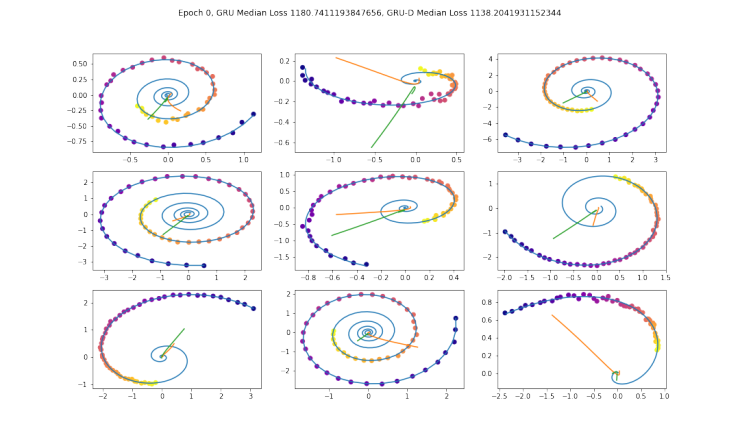
\includegraphics[scale=0.25]{vis0.png}
    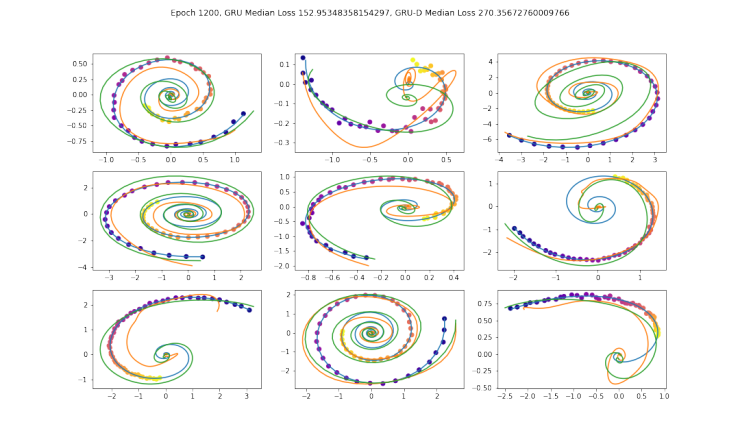
\includegraphics[scale=0.25]{vis1200.png}
    \caption{Before (left) and after (right) training for 1200 epochs on the spiral dataset}
    \label{fig:my_label}
\end{figure}

\section{Methodology}
\subsection{Data Preprocessing}

The training data was readily available using the Kaggle API and can be found at \url{https://www.kaggle.com/c/web-traffic-time-series-forecasting/data}. The data is made up of a page column, containing a concatenation of the article name, type of traffic, and crawling agents used to obtain data, as well as the number of page hits for each day between July 1st, 2015 and December 31st, 2015. Empty values are used to represent missing data (note that missing here can either mean the traffic was zero or that the data was not available for that day). The training data consists of a total of 145,063 websites and 803 time points in total.
\begin{figure}[h]
  \centering
  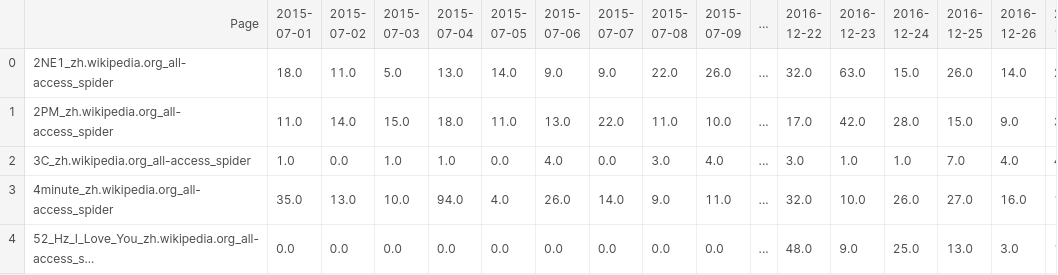
\includegraphics[width=13cm]{train_overview.png}
  \caption{First 5 pages of training data}
\end{figure}

We first preprocess our data by converting it to a PyTorch tensor and using the methods described below to account for missing data. First, we remove any rows where more than 10\% of the time points have missing data. This is to shrink the training dataset so that the model only trains on web traffic data with sufficient data points to allow effective fitting of an ODE.

Next, we use various interpolation methods to remove the missing time points in the remaining rows. Among the interpolation methods we used were a zero-based interpolation (each NaN value in the dataset is replaced by a 0), a median-based interpolation (each NaN value in the dataset is replaced by the median of the row), a mean-based interpolation (each NaN value in the dataset is replaced by the mean of the row), and a mean-based interpolation with noise (each NaN value in the dataset is replaced by a value normally distributed around the mean of the row). For models made using a GRU-D, we don't perform any of the above interpolations and directly feed in data containing the NaN values. Among the models using the above interpolation methods, the best-performing model was obtained with a median-based interpolation. We discuss possible reasons for why this may be further below.

\subsection{Model Architecture}

Our final model architecture consists of a variational autoencoder, where the encoder block is a GRU-D cell and the decoder block is a latent neural ODE. The encoder block generates a latent space representation of an ODE for the time series data and the decoder block essentially integrates over this ODE to obtain a prediction for any time value given an initial time. We use a learning rate of 0.001, train on a random sampling of 200 timesteps, batch size of 1000, and the Adam optimizer.

\begin{figure}[h]
  \centering
  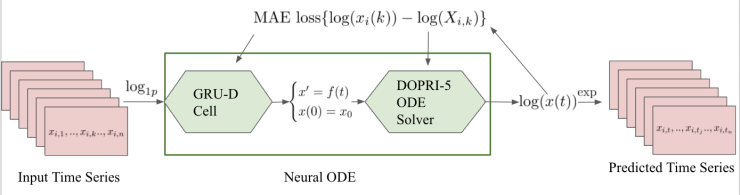
\includegraphics[width=10cm]{architecture.png}
  \caption{Latent ODE model with GRU-D encoder}
\end{figure}

The GRU-D cell is implemented from scratch and can be called in exactly the same way as the GRU cell. A PyTorch implementation of the GRU-D cell is given in the publicly available repository since other publicly available implementations are either buggy or hardcoded for time series classification problems rather than time series forecasting problems.

A high-level overview of a GRU vs GRU-D cell is provided below:
\begin{figure}[h]
  \centering 
  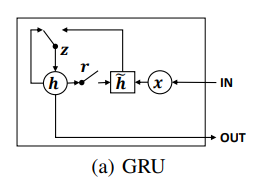
\includegraphics[width=5cm]{gru.png}
  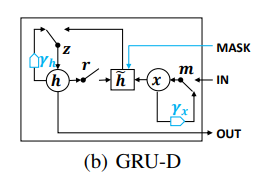
\includegraphics[width=5cm]{grud.png}
  \caption{Graphical Illustrations of GRU vs. GRU-D models}
\end{figure}

Essentially, a GRU-D uses a mask to filter out missing input values as they are fed to the network. However, these missing values are replaced by the output of a hidden layer that extrapolates these values based on previous data fed to the network. A GRU-D allows for far more flexibility it interpolation since it dynamically trains a neural network to calculate missing values rather than using a fixed method such as zero, median, or mean interpolation.

The latent ODE decoder determines a trajectory from the initial hidden state $z_{t_0}$ output by the encoder and uses it to predict $z_{t_1}, \ldots, z_{t_n}$. 
We specifically use a DOPRI 5 solver to integrate the ODE. After experimentation with solvers including the Euler's method, Dopri5, Dopri8, Adams Bashfroth Moulton, Midpoint, and the built-in scipy solver, we found that Dopri5 was the best. This is likely because Dopri5, Dopri8, and the built-in scipy solver are able to account for the greatest stiffness in data and thus, allow for use of higher learning rates with lower batch sizes.
\begin{figure}[h]
  \centering
  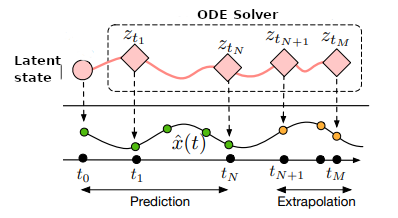
\includegraphics[width=8cm]{decoder.png}
  \caption{Latent ODE decoder architecture}
\end{figure}

\subsection{Training Method}

We train by shuffling the rows in the training data to obtain a random permutation of websites for each epoch. For each row in a batch, we then sample $n$ timepoints starting from a random date between July 1st, 2015 and December 31st, 2015. We experimented with randomly dropping timepoints to create non-continuous data but found that, while this didn't make a substantial difference for the training loss, it lead to inefficient generalization to the testing data. Additionally, it outweighed the benefits of any given interpolation method and as such, we decided to feed in continuous time data after interpolation was performed (for the GRU).

\subsection{Loss Methods}

Particularly difficult was finding a loss function that could be minimized. Although the test predictions are evaluated using a SMAPE loss, such a loss is difficult to optimize since the value of the function near 0 is undefined. As a result, we experimented with other loss functions including MSE, MAE, a differentiable version of SMAPE, a rounded version of SMAPE, and MAPE. Comparisons between each of these functions are shown below:
\begin{figure}[h]
  \centering
  \centering
  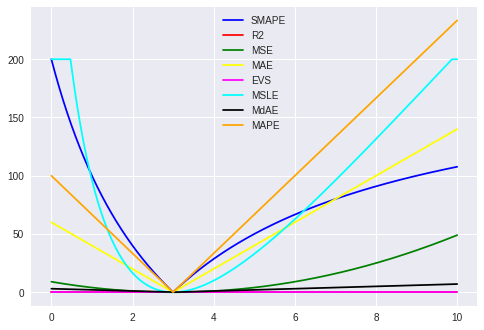
\includegraphics[width=6cm]{loss_0.png}
  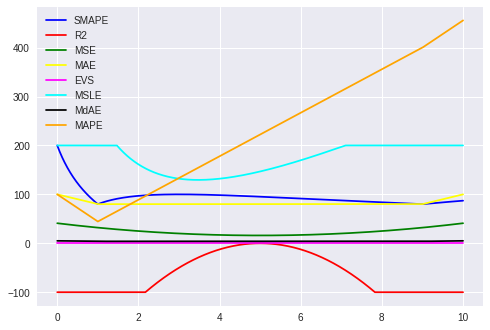
\includegraphics[width=6cm]{loss_1.png}
  \caption{Loss Function Comparison}
\end{figure}

We found that performing a log1p transformation on the data before applying the MAE loss function allowed us to minimize the loss function optimally. This is because a log1p transformation decreases the magnitude of the data points, allowing for more continual training of the model given data containing sudden spikes in web traffic. The MAE loss function smoothes the results at most data points, providing a similar function. Given that the MAE loss is close to the SMAPE competition loss function, it is an efficient substitute for training.

\section{Results}
We obtained a final SMAPE score of 41.2. For reference, the top submission on Kaggle which uses a Seq2Seq model achieves a SMAPE score of 35.48, where lower values are more accurate. We train with about half the amount of parameters compared to the top submission (28838 vs 50116) and also with 125 epochs (125 gradient updates per epoch) vs 10,000 epochs (20 gradient updates per epoch). 
Trained for a greater number of epochs, it is likely that our model could achieve a sub-40 SMAPE score. Given the large difference in the number of parameters and training time, there is significant evidence that neural ODEs are better able to forecast time series data, particularly when significant portions are missing. 

Training took roughly 4 hours per model, 10 seconds per batch with GRU, and 12 seconds per batch with GRU-D. Below, we plot the final SMAPE scores for twelve different models, with each model trained on a different combination of encoder architecture (GRU vs. GRU-D) and loss function (MAE, MSE, or differentiable SMAPE).
\begin{figure}[h]
  \centering
  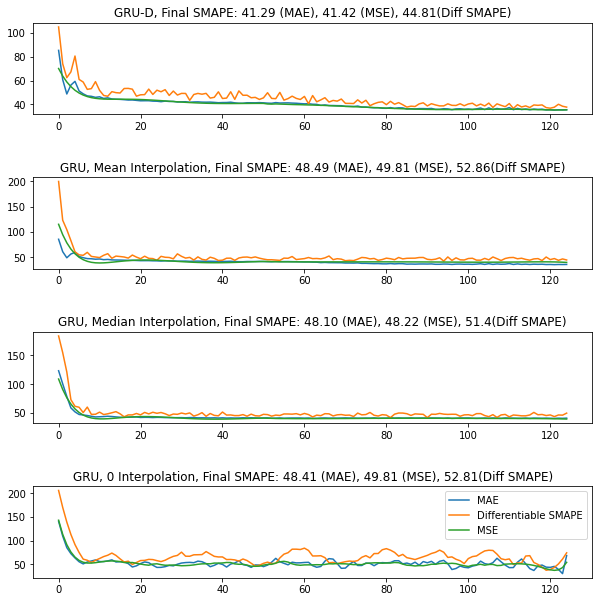
\includegraphics[width=9cm]{losses.png}
  \caption{Final SMAPE scores for 12 different models}
\end{figure}

We also experimented with different ODE solvers for the GRU-D architecture and an MAE loss. Among the solvers we tried were the DOPRI-5, DOPRI-8, Scipy Solver, Adams Bashforth Moulton, Midpoint, and Euler solvers. 
\begin{figure}[h]
  \centering
  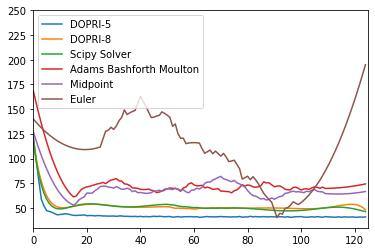
\includegraphics[width=8cm]{solvers.png}
  \caption{SMAPE scores with different ODE solvers}
\end{figure}

\newpage
Below, we display the results of our model predictions versus the actual web traffic values for selected samples. Note that the predictions are typically smoother as a result of the shape of the MAE loss function as well as the ODE solver.
\begin{figure}[h]
  \centering
  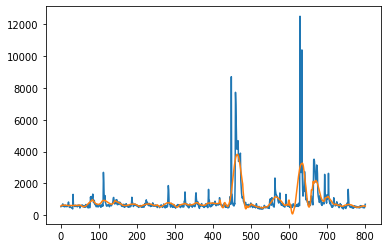
\includegraphics[width=6cm]{predict1.png}
  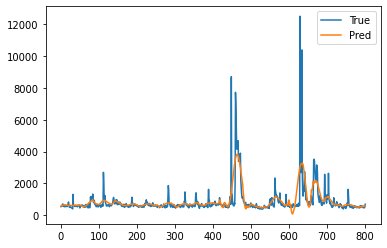
\includegraphics[width=6cm]{predict2.png}
  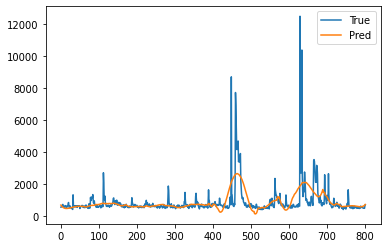
\includegraphics[width=6cm]{predict3.png}
  \caption{Model predictions vs. actual time series data}
\end{figure}

\section{Challenges}
The point of the dataset was to try and develop a method for fitting very noisy, jagged, and irregularly sampled data. This is one of the most challenging characterizations of time series, and as a result we had to research and employ a myriad of techniques to allow our model to effectively fit and predict the data. We split up our challenges and solutions into 3 main categories:
Data Processing:
Since the data had many large peaks it made training impossible since the model would both attempt to fit the low average traffic and peak traffic. As a result, we initially employed outlier exclusion, but this effectively prevented the model from learning at all. We also employed average window smoothing, but this caused the same issue. As a result we chose to just log transform the input, so our model would train in log space, drastically reducing the euclidean distance between the peak and maximal value. Also, many websites had extremely large gaps in between data entries, roughly 20\% of the entire time series would be NaNs in these cases, as a result, we excluded these websites from training overall, and then trained a separate model with its own weights to fit particularly on these websites. Here the GRU-D based models exceptionally outperformed the GRU models since interpolation methods effectively erased any possible trends to be extrapolated from the gaps. Interpolation methods themselves were a pitfall, initially we were not adding any random noise and as a result the models performed exceptionally well in training but had poor extrapolation performance on the test data sets. We tried different distributions, but found uniform distribution led to the best performance. We tested this by removing random points, replacing the missing points with the interpolation with different noises (Gaussian, Xaviar, Exponential, Uniform) and we found uniform produced the lowest KL-divergence.

\subsection{Training}
The train time was the most exceptional difficulty, since two of our group members could not run the model locally, we were limited to 6 devices counting the free GCP accounts each of us made. This meant we had to be careful about setting up and running experiments since training took roughly 4 hours. Each batch took about 10 seconds to train for GRU models and 12 seconds for GRU-D models, we used batch size = 1000, and there are roughly 144,000 websites. We also had a lot of difficulty setting up Cuda for both the GRU and GRU-D based model, so we were unable to take advantage of GPUs in our training. While the loss profile seemingly indicates convergence, the model actually becomes much more accurate even past 100 epochs. In our literature review, most experiments trained for over 1000-10,000 epochs, but this would take over 2 weeks by our calculations without Cuda, so we settled on a realistic amount of epochs for experiments and trained for a whole day for our final model which we submitted on Kaggle. 

\subsection{Testing}
The model initially had really poor testing performance due to overfitting. Using a 10-fold cross validation to optimize hyperparameters alleviated the issue, but the most significant improvement came from implementing dropout. We suspect applying gentler smoothing techniques than average window such as Savitzky-Golay filtering would improve generalizability too. 

\section{Reflection}
The model worked out the way we expected it to. We were able to apply NeuralODEs to incredibly difficult time series forecasting problems, achieving near state of the art results. We did this using GRU-D’s powerful interpolation capabilities, along with methods such as dropout and input transform/normalization. We have achieved a 41.21 SMAPE evaluation score which places us at the higher percentile on the official kaggle public leaderboard. Overall, we are satisfied with the results achieved by the model and are close to achieving our specified target goal.

Our initial approach was using a SMAPE loss as a loss function. Upon realizing that using SMAPE as a loss function causes unstable behavior near zero values, we transitioned over to training the model on the MAE loss function (Mean Absolute Error) by feeding it log transformed data. This produces smoothed results at most data points. If we were to do the project all over again, we would have tried a more complex preprocessing framework that would allow us to account for interpolations at every day of the week instead of simply taking interpolations for each week. This would have produced deeper comparisons against our GRU-D method.

In addition to considerations mentioned above such as Savitzky-Golar filtering, training for longer, and adding Cuda capabilities, we are also very interested in latent PDE generation rather than latent ODE. This is because while our system of ODEs representation does well, it fails to effectively capture relationships between websites. Intuitively it makes sense for related topics or articles in the same language to have somewhat related traffic. We theorize that making each website a dimension of a latent PDE and using PDE solving techniques could also be fruitful. 

The biggest takeaway from this project is the importance of cross validation. Since we are dealing with an irregular dataset, we would have to consider other methods of interpolation on nan values. This includes median, mean, and zero interpolation, and finally an implementation of GRU-D which instead accounts for these nan values and trains on them. We have done testing on these methods and found that our intuition on GRU-D is correct and would produce the most accurate results. Another takeaway is the importance of looking at our current solutions from a practical standpoint. For example, is including nan values in training feasible? We did some thinking on the problem at hand and concluded that missing values could be a form of informative missingness (eg. anomalies/inconvenience). This means that by addressing missing values in the time series, we would be able to achieve better results.

\section{Related Work}
The original paper for this work, Neural Ordinary Differential Equations (https://arxiv.org/pdf/1806.07366.pdf) lays out three main benefits of neural ODES:
\begin{itemize}
  \item They have a constant memory cost, allowing for training of deeper models.
  \item Adaptive computation allows for an accuracy vs. time tradeoff
  \item Applicable to continuously-defined dynamics
\end{itemize}

In this paper, the authors actually mention that applying traditional neural networks to irregularly-sampled data such as network traffic is difficult but that neural ODEs present a continuous-time, generative approach that may provide significant improvements. However, we have not found any papers since then that lay out the architecture of such a model and evaluate its performance against a test dataset.

Neural ODEs have successfully been applied to other time-series data though. For example, they have been used to successfully predict the weather in Delhi based only on a dataset of climate measurements over the past few years (https://sebastiancallh.github.io/post/neural-ode-weather-forecast/).

Additionally, there are numerous articles discussing potential variations on the basic neural ODE architecture described by Ricky Chen et. al in the original paper such as ODE-RNN hybrids and latent ODEs (https://proceedings.neurips.cc/paper/2019/file/42a6845a557bef704ad8ac9cb4461d43-Paper.pdf) that provide ample opportunity for fine-tuning of model parameters and potentially creation of a novel architecture specific to this problem.

The original paper for GRU-D (https://arxiv.org/pdf/1606.01865.pdf)

In this paper, the authors points out that missing time steps in temporal data would count as a valuable observation. Instead of filling in missing values, masking is used to inform the model on missing data and time intervals are used to observe input patterns. By considering these dependencies and training on all components through back propagation, using GRU-D would greatly improve the model's accuracy.

Given the existing theoretical background as well as effective, albeit limited, papers applying neural ODEs to other time-series data, this presents an exciting opportunity to explore the potential of neural ODEs with a GRU-D encoder for irregularly sampled datasets.

\end{document}